\FloatBarrier
\section{Software stack and cross-platform application}\label{sec:software}

\subsection{Requirements}
A domain-specific accelerator fails if it is hard to program. \ac{1} is designed for a small set
of kernels and the software stack reflects that: rather than a general programming model, it
exposes a library of atmospheric formulas behind one-line calls, and a compilation path that maps
those formulas onto the tile array without the user ever writing AVISA. The stack has four
requirements.

\begin{enumerate}[leftmargin=1.4em,itemsep=1pt]
\item \textbf{One line per physical problem.} A forecast, an ensemble analysis, a Lyapunov
      spectrum or a dispersion calculation should be a single function call with named
      parameters.
\item \textbf{The same call on every platform.} macOS (Apple silicon and Intel), Windows and Linux,
      from Python, JavaScript, a command line and a graphical application.
\item \textbf{Inspectable execution.} Because the schedule is static, the runtime can report the
      cycle count, the energy per block and the precision coverage of a run before it finishes.
      The application shows these numbers rather than hiding them.
\item \textbf{Reproducibility.} A run is identified by its formula, parameters and seeds, and can
      be replayed bit-for-bit.
\end{enumerate}

\subsection{Stack overview}
Fig.~\ref{fig:software}(a) shows the four layers. The application and the SDKs never touch the
device directly; they issue jobs to the driver, which validates parameters, allocates buffers,
programs the tile array and streams telemetry. The driver exposes seven calls
(Fig.~\ref{fig:software}(d)); the same seven are implemented by the virtual device that ships with
this report and by the silicon driver, so code written against the application runs unchanged on
hardware.

\subsection{Compiler and runtime}
The compilation flow is shown in Fig.~\ref{fig:software}(b). An atmospheric program is written in
a small dataflow DSL in which stencils, ensemble reductions, observation operators and physics
packages are primitives. The compiler lowers it to ACPU-IR, maps it onto 3D tile blocks with
explicit halos, plans per-cell precision classes from the spread field and statically schedules
each tile. The output is an AVISA binary plus a halo script.

Because there is no dynamic scheduling, the scheduler can compute the exact cycle count of a tile
before the run. For the reference step it is 61,900 cycles; the application displays this number
and the corresponding worst-case execution time, which is what makes the response-time claims of
Section~\ref{sec:deployment} meaningful.

\begin{figure}[t]
\centering
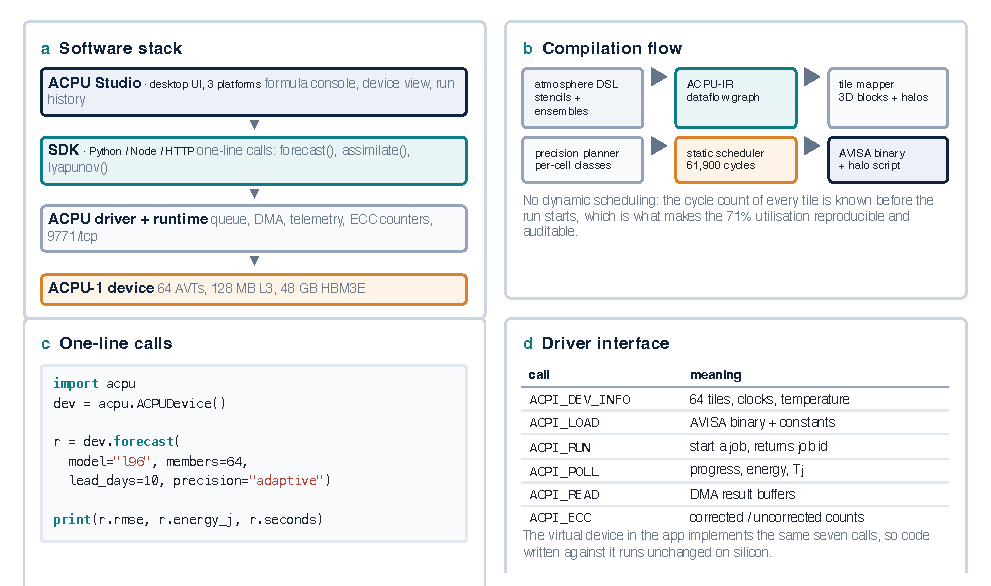
\includegraphics[width=\linewidth]{fig23_software}
\caption{Software stack. (a) Four layers from application to device. (b) Compilation flow from the
atmosphere DSL to an AVISA binary. (c) A one-line call in Python. (d) The seven-call driver ABI.}
\label{fig:software}
\end{figure}

\subsection{SDK interface}
The Python SDK is dependency-free and speaks HTTP to the device service, so it works from a
notebook, a batch script or a cluster login node. The same surface is available in JavaScript for
web and Electron clients, and on the command line.

\begin{verbatim}
import acpu

dev = acpu.ACPUDevice()                      # connects to 127.0.0.1:9771
print(dev.status())                          # 64 tiles, 1.80 GHz, 57 W, 74 C

run = dev.forecast(model="l96", members=64, lead_days=10,
                   precision="adaptive", time_budget_s=30)
print(run.rmse, run.energy_j, run.seconds)   # 1.33  7174.9  125.6

spec = dev.lyapunov(model="l96", n_exp=12)   # leading exponents
map_ = dev.transport(source=(22.75, 113.57), hours=6, resolution_km=3)
\end{verbatim}

The design rule for the parameter set is that every argument has a physical unit and a default
that is meaningful for an operational user: \code{members}, \code{lead\_days},
\code{precision}, \code{time\_budget\_s}. There is no device-specific tuning parameter in the
public API; the clock, the precision policy and the tile mapping are chosen by the runtime from
the time budget and the requested skill.

\subsection{ACPU Studio}
ACPU Studio is the cross-platform desktop application that ships with this report. It is an
Electron application with no external runtime dependencies, built for macOS (universal binary),
Windows (installer and portable) and Linux (AppImage and tarball). It embeds the virtual device,
so it runs a complete ensemble forecast on a laptop without any hardware.

The interface is designed as a scientific instrument panel rather than a dashboard. The console
view (Fig.~\ref{fig:ui}(a)) pairs a formula library with a parameter form and a generated call,
so that the same operation is available as a GUI form, a one-line call and a reproducible
parameter record. A run streams telemetry at 10 Hz: per-cluster utilisation, power, junction
temperature and memory bandwidth (Fig.~\ref{fig:ui}(c)). Results are shown as charts with the
device metrics alongside them (Fig.~\ref{fig:ui}(b)), because the point of the machine is the
ratio between the two. The runs view keeps a history of executions with their exact parameters and
seeds; the documentation view carries the API reference and code samples for Python, JavaScript
and HTTP (Fig.~\ref{fig:ui}(d,e)).

\begin{figure}[t]
\centering
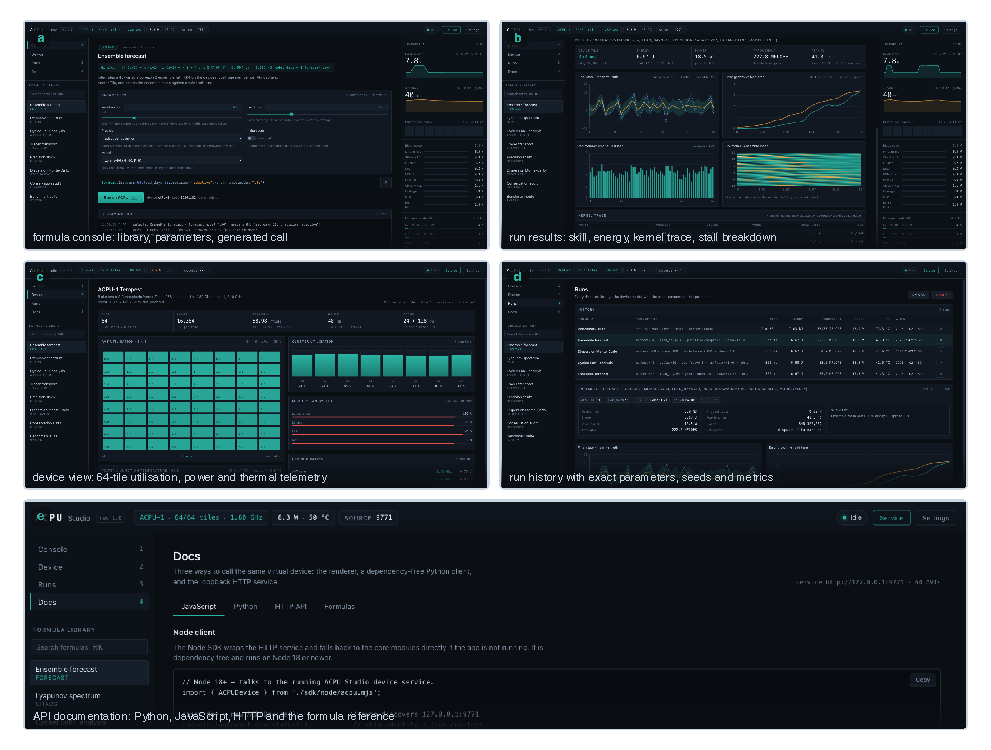
\includegraphics[width=\linewidth]{fig24_ui}
\caption{ACPU Studio. (a) Formula console with parameter form and generated call. (b) Run results
with skill and device metrics. (c) Device view: 64-tile utilisation map, power and temperature
telemetry. (d) Run history. (e) API documentation. Screenshots from the packaged application.}
\label{fig:ui}
\end{figure}

\subsection{Validation of the software}
The application is tested at three levels. A headless self-test runs every formula, asserts that
outputs are finite and within physical bounds, and prints a pass table. A screenshot harness
drives the real window over the Chrome DevTools Protocol, exercises the console, runs a forecast
and captures the five views used in Fig.~\ref{fig:ui}. The SDK is tested against the running
application over HTTP, from both Python and Node, including error paths (unknown parameter,
out-of-range member count, device not running).

The virtual device is not a hardware emulator. It implements the same formulas, the same
precision modes and a calibrated model of the device's cycle and energy counters, but it computes
in JavaScript on the host CPU and its timings are simulated, not measured. It exists so that the
API, the UI and the numerical pipeline can be developed and reviewed before silicon, and the
report is explicit that the numbers it produces in the application are model numbers, consistent
with those in Section~\ref{sec:results} by construction.
